%----------------------------------------------------------------------------------------
%	RESULTS 1150 words
%----------------------------------------------------------------------------------------
\section{Results}

\subsection{Flux Tower Site Clustering}
Cluster analysis was carried out in order to classify sites into groups based on their characteristics. This classification permits the predictability of ET, both within these characterised groups and across them, to be investigated. Gower's distances \parencite{gower1971} were computed as a measure of dissimilarity between all site pairs using the features listed in \autoref{tab:cluster_vars} and saved as a matrix. This matrix was then passed to the Partitioning Around Medoids (PAM) algorithm \parencite{rousseeuw1990} with the silhouette method to form clusters and identify medoid sites - those which have minimal dissimilarity to other sites within each cluster and thus can be seen as representatives of each cluster.\par The silhouette method identified $k = 13$ as the optimal number of clusters based on average silhouette width, but with only 51 sites present this value was dropped to $k = 6$ in order to yield sufficiently well-populated clusters across a range of site characteristics. The cluster assignment solution from PAM with $k = 6$ clusters resulted in a range of site counts by cluster from 3 sites (cluster 6) up to 18 sites (cluster 3), and can be seen in a cluster plot of the first two principal components (\autoref{fig:cluster}). The six medoid sites were geographically distributed with four sites in North America and two sites in Europe (\autoref{fig:map}), and a range of site ages from 20 years (US-Me3) up to 117 years (DE-Lnf). 

 \par To define cluster site characteristics, the means of z-score standardised (mean = 0, sd = 1) numerical features and mode of categorical features were considered for each cluster. Mean scaled numeric features can be seen within a heat map (\autoref{fig:pheat}) for a visual comparison across clusters. Mean cluster features $\geq$ 1 sd from the all site mean were considered as `high/low' ($\geq$ 1.5 sd as `very high/very low') in order to qualitatively classify cluster characteristics, with these summarised in \autoref{tab:cluster_characteristics}.


\begin{figure}[H]
	\fbox{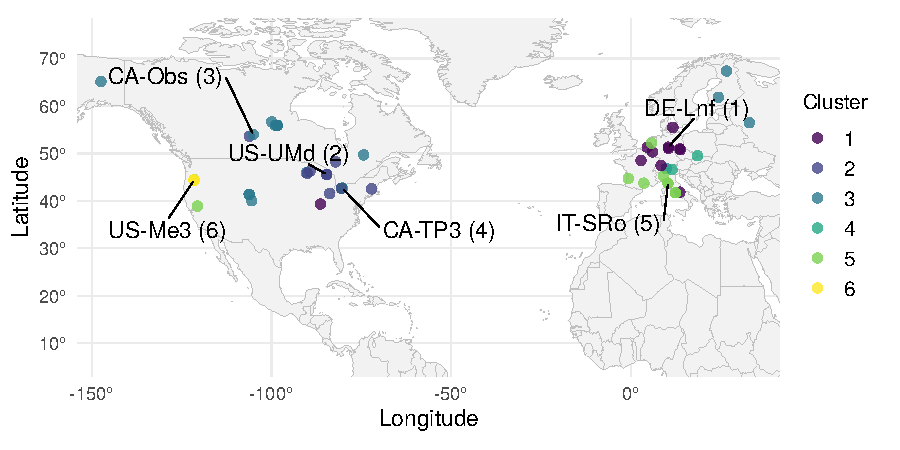
\includegraphics[width=\linewidth]{../../figures/world_sites_clusters.pdf}}
	\captionsetup{justification=centering}
	\caption{Map of FLUXNET sites and associated clusters in this study, with cluster medoid site IDs highlighted. The geographic distribution of clusters follows an expected pattern with regards to climate site. CHANGE/ADAPT}
	\label{fig:map}
\end{figure}

\begin{figure}[H]
	\fbox{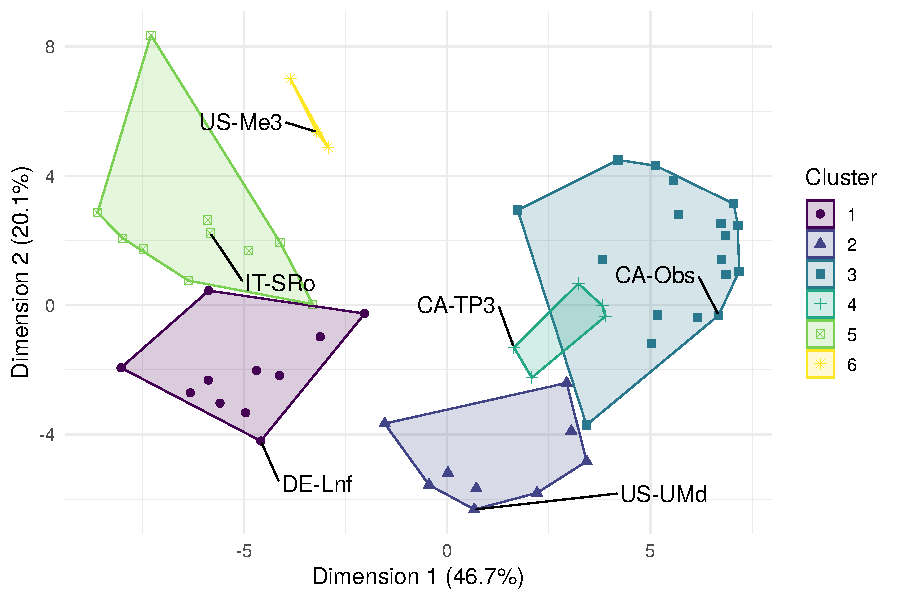
\includegraphics[width=\linewidth]{../../figures/cluster_plot.pdf}}
	\captionsetup{justification=centering}
	\caption{Cluster plot indicating the site positions in the space of the first two principal components, with coloured clusters indicating the PAM solution. Axes indicate percentage of variance explained by each dimension.}
	\label{fig:cluster}
\end{figure}

\begin{figure}[H]
	\fbox{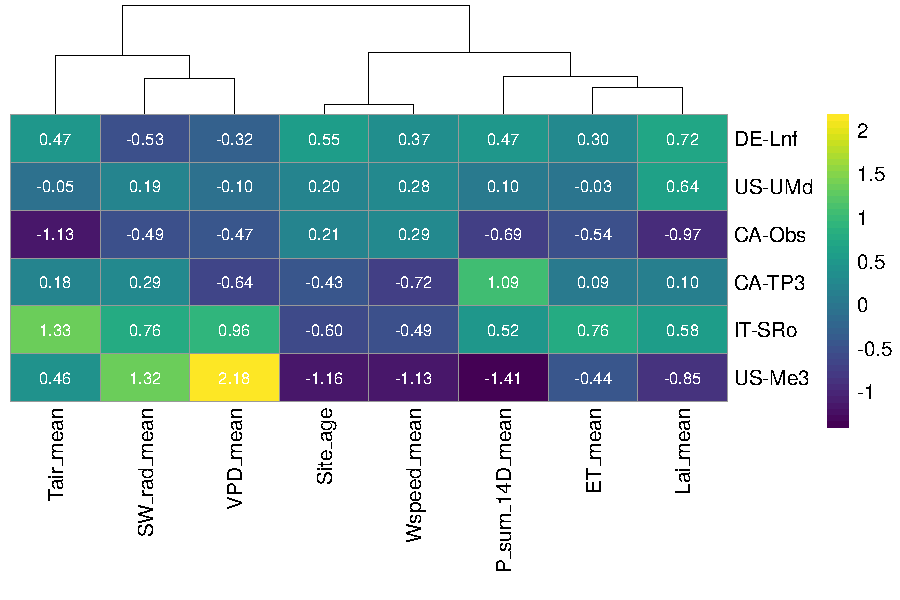
\includegraphics[width=\linewidth]{../../figures/pheat2.pdf}}
	\captionsetup{justification=centering}
	\caption{Heatmap of cluster medoid sites and scaled feature values. Scaled features $\geq$ 1.5 standard deviations from the mean of all sites were classed as 'very' (high or low, depending on direction), while features between 1 and 1.5 standard deviations from the mean were classed as high or low, depending on direction, in order to characterise clusters.}
	\label{fig:pheat}
\end{figure}

\begin{table}[hbt]
	\caption{\centering Main characteristics of each cluster defined during cluster analysis}
	\centering
	\begin{tabularx}{\linewidth}{llXl}
		\toprule
		Cluster & Medoid Site & Defining Characteristics \\
		\midrule
		1 & DE-Lnf & Temperate sites without significant features.  \\
		2 & US-UMd & Continental sites without significant features. \\
		3 & CA-Obs & Continental sites with low mean air temperatures.  \\
		4 & CA-TP3 & Continental sites with high precipitation.  \\
		5 & IT-SRo & Temperate sites with high air temperatures.  \\
		6 & US-Me3 & Temperate sites with very high VPD, high SW radiation, low stand age, low wind speeds, and low precipitation. \\
	\end{tabularx}
	\label{tab:cluster_characteristics}
\end{table}


\subsection{Spatial Generalisation}

%Suggested framing:

%US-UMd (age helps) vs De-Lnf (age hurts) as case studies


%For each: SHAP dependence plot for age, feature importance ranking, brief site characteristics (climate, age, cluster membership)
%Then the permutation test as a cross-cutting check — not per-site, but run once (or per-cluster) across the whole train/test setup to test whether age's apparent value is real signal or site-proxy leakage

%Mention the other 4 clusters exist and were tested (maybe one summary table/plot of all 6 site R² deltas) so it's clear you didn't cherry-pick — then justify the deep dive as case studies. That's a normal, well-scoped move for a 4k-word section, not weak coverage.


%Spatial (bulk of results): cluster analysis overview (brief, all 6), then deep dive on DE-Tha vs CA-Obs (SHAP, feature importance, why age helps/hurts), permutation test as the credibility check
%Temporal: shorter section — does age still help/hurt over time at a couple of long-record sites, tying back to the leakage question (age varies within-site here, so it's a cleaner test)
%Discussion: synthesize — when/why age helps, leakage risk, what it means for future FLUXNET+age model building

\subsubsection{Analysis 1.1 - Model Sensitivity} \label{model_sens}

\begin{figure}[H]
	\fbox{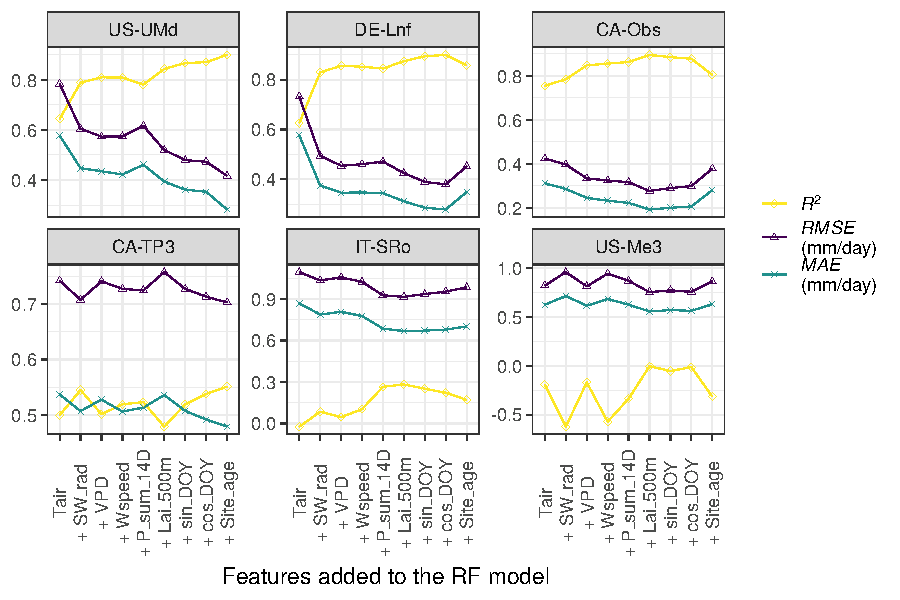
\includegraphics[width=\linewidth]{../../figures/1.1_p1.pdf}}
	\captionsetup{justification=centering}
	\caption{R$^2$, RMSE, and MAE for medoid cluster site predictions of ET (ordered left-right and top-bottom) by peak R$^2$ with clusters indicated in facet names. Models built and tested using a consecutively greater number of input features from FLUXNET and LAI data (the `+VPD model' incorporates Tair, SW\_rad, and VPD as training and input features here). R$^2$ performance at only half of the sites was good, and suggests that adding features up to site age improved prediction accuracy at four of the six medoid sites. Adding age as a final feature led to mixed performance CHANGES across the medoid sites.}
	\label{fig:adding_features}
\end{figure}

\subsubsection{Analysis 1.2 - Shuffled Training Sets}


\begin{figure}[H]
	\fbox{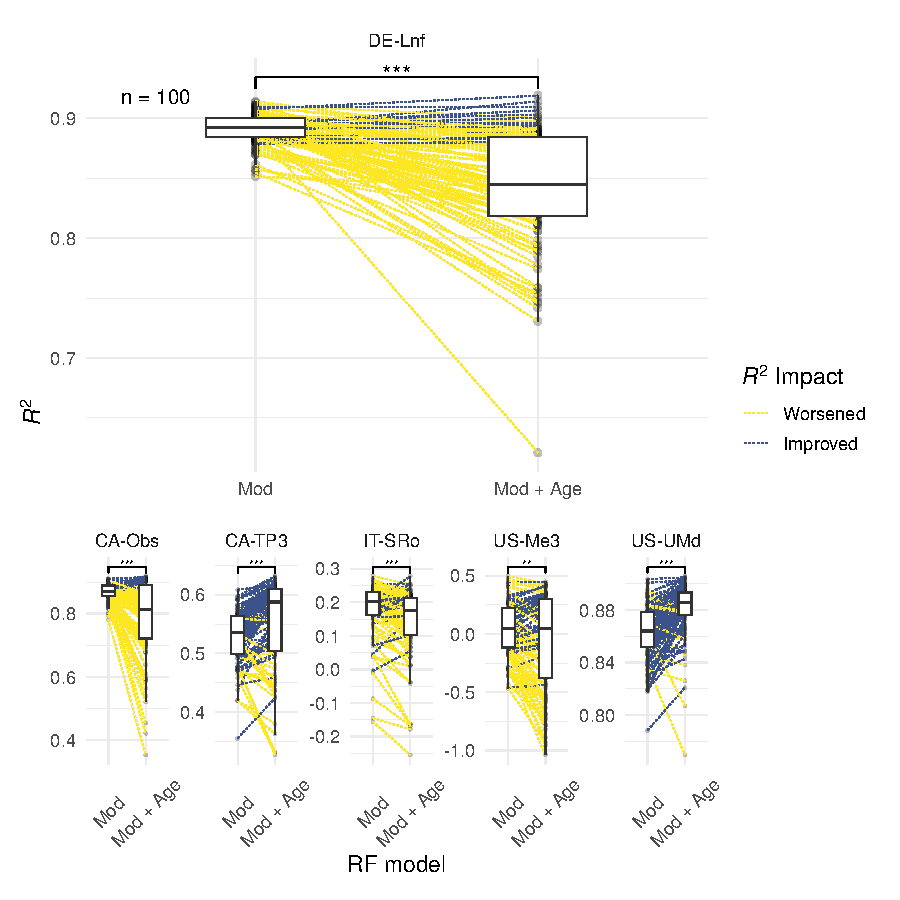
\includegraphics[width=\linewidth]{../../figures/1.2_p3.pdf}}
	\captionsetup{justification=centering}
	\caption{Paired box-plots indicate the impact on R$^2$ when age is added as a feature to RF models across 100 repeated runs of randomly sampled training datasets. Points are connected on a per-run basis where training dataset site composition is identical. Wilcoxon signed-rank tests suggest model performances differ significantly at all test sites. DE-Lnf is shown large for readability, with other cluster medoid sites shown at a reduced scale for comparison.}
	\label{fig:paired_box}
\end{figure}

\paragraph{Training Set Compositions} Here I will quickly look into the training set compositions of the RF models where age improved OR worsened R$^2$.

\begin{figure}[H]
	\fbox{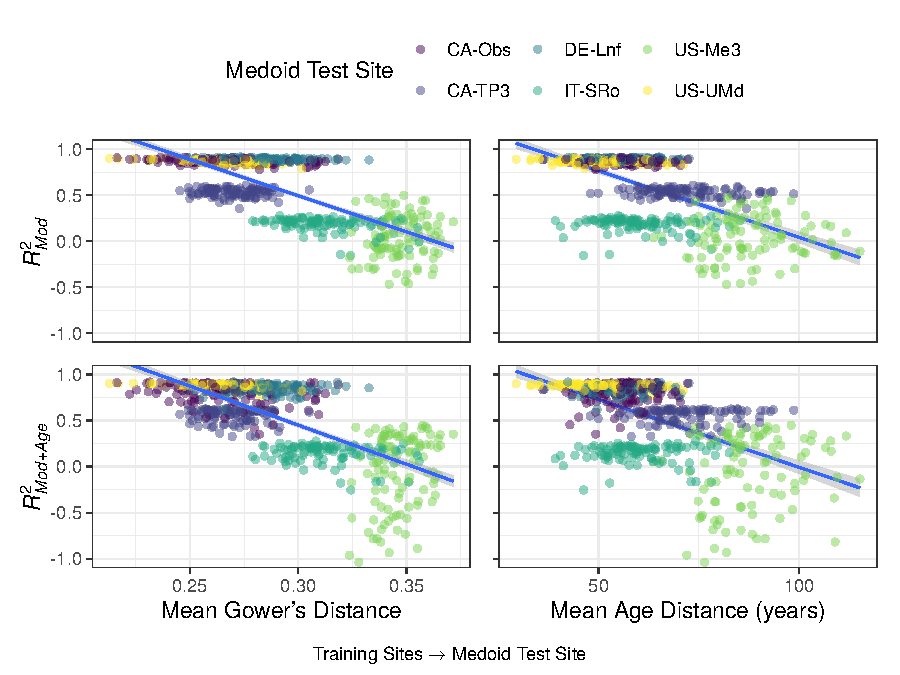
\includegraphics[width=\linewidth]{../../figures/1.2_gower_r2.pdf}}
	\captionsetup{justification=centering}
	\caption{Plots }
	\label{fig:r2_gower}
\end{figure}


\subsection{Temporal Generalisation}


\subsection{Case Study of US-UMd and DE-Lnf}

- Look into predictions vs observed at both this R2 plot but also over timeframe  \\
- US-UMd: Continental Site, 2715 days of data, 90 years old \\
- DE-Lnf: Temperate Site, 2670 days of data, 117 years old

\begin{figure}[H]
	\fbox{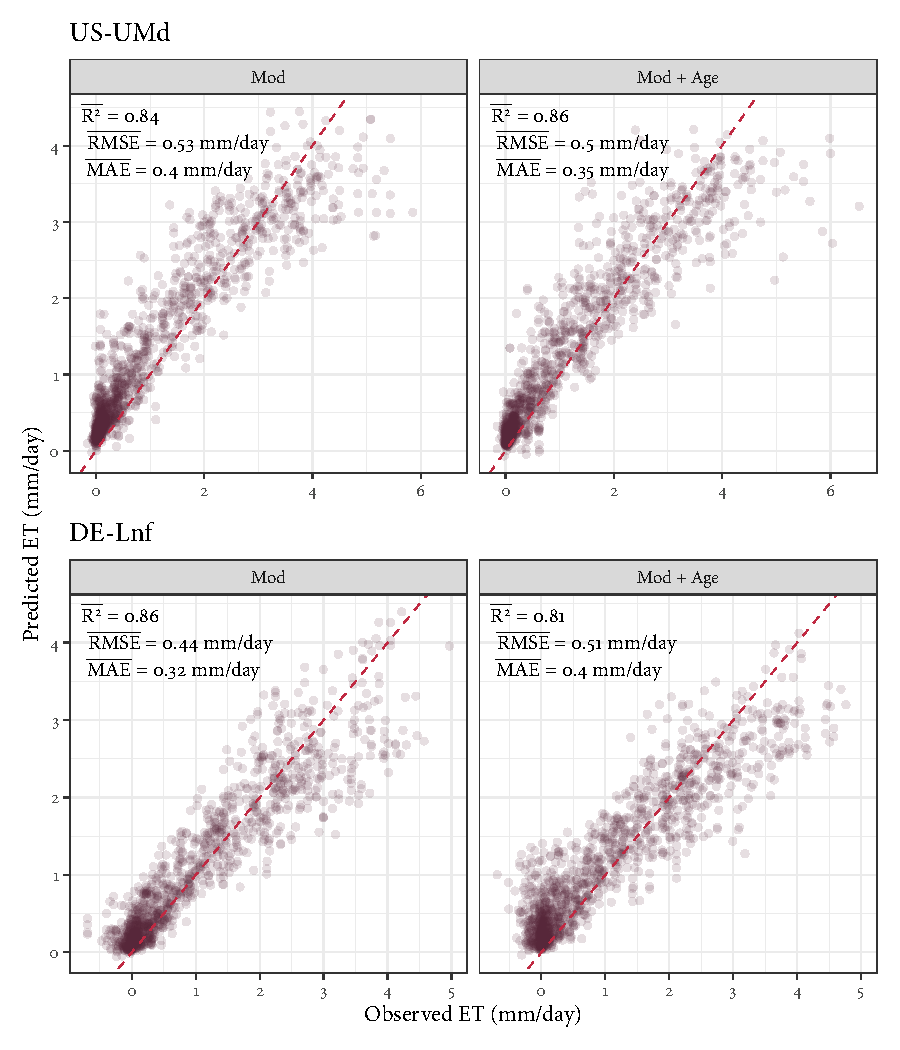
\includegraphics[width=\linewidth]{../../figures/1.2_merged1.pdf}}
	\captionsetup{justification=centering}
	\caption{Subset of 2500 data points}
	\label{fig:pred_obs}
\end{figure}

\begin{figure}[H]
	\fbox{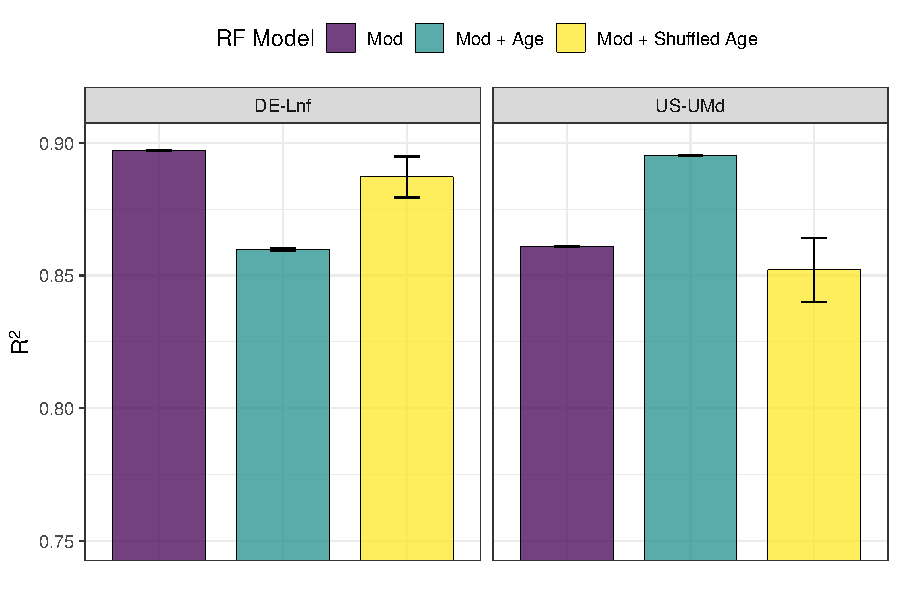
\includegraphics[width=\linewidth]{../../figures/case_study_bars.pdf}}
	\captionsetup{justification=centering}
	\caption{Bar plot showing the effect of different model setups on R$^2$ at DE-Lnf and US-UMd, with error bars indicating standard error. Models were trained using a leave one group out (LOGO) approach, with ten repeats using different \texttt{NumPy} seeds. To assess whether site age was acting as a proxy for other site-level characteristics in these models, a model which randomly shuffled ages between sites was also formed using identical seeds and LOGO approach. This `shuffled age' model appeared to increase R$^2$ at DE-Lnf compared to the Mod + Age model where an opposite effect was observed at US-UMd, suggesting that true age-ET relationships learned by the model transfer well to predicting ET at US-UMd, but not at DE-Lnf.}
	\label{fig:case_study_bars}
\end{figure}

